\chapter{Efficient Algorithm Selection}
\label{chapter:alphalinkage}

\todo[inline]{more formal definitions and lemmas}

We define $\alpha$ as the parameter with which the output of an algorithm is weighted. In this chapter we propose different distance measures depending on the weight parameter $\alpha$ that allows us interpolating between different linkage strategies in a way similar to the proposed by Balcan et al. \cite{DBLP:journals/corr/BalcanNVW16}, where a infinite interval was proposed.

To have a real application, we need to have a finite set of intervals. So we interpolate between one algorithm with $\alpha = 0$ and another algorithm with $\alpha = 1$, where for $\alpha = 0$ the result will be the result of algorithm 1 and for $\alpha = 1$ the result of algorithm 2.

\section{Linear Interpolation between two different linkage strategies}

Interpolating between two of the three mentioned linkage strategies results in three different algorithmic settings. In the first setting we are using the single linkage distance $d_{SL}(X,Y)$ and the complete linkage distance $d_{CL}(X,Y)$. By combining the two distances we can create a linear model that ranges from $\alpha = 0$ (single linkage) to $\alpha = 1$ (complete linkage) resulting in equation \ref{eq:singlecomplete}.

\begin{equation}
    \begin{aligned}
        \dsc(X,Y,\alpha) &= (1 - \alpha) \cdot d_{SL}(X,Y) + \alpha \cdot d_{CL}(X,Y)\\
        &= (1 - \alpha) \min\limits_{x \in X, y \in Y} d(x,y) + \alpha \max\limits_{x \in X, y \in Y} d(x,y)
    \end{aligned}
    \label{eq:singlecomplete}
\end{equation}

Equivalently we can interpolate between the single linkage distance $d_{SL}(X,Y)$ and the average linkage distance $d_{AL}(X,Y)$ instead of the complete linkage distance $d_{CL}(X,Y)$ for $\alpha = 1$ resulting in equation \ref{eq:singleaverage}. 

\begin{equation}
    \begin{aligned}
        \dsa(X,Y,\alpha) &= (1 - \alpha) \cdot d_{SL}(X,Y) + \alpha \cdot d_{AL}(X,Y)\\
        &= (1 - \alpha) \min\limits_{x \in X, y \in Y} d(x,y) + \alpha \frac{1}{|X| |Y|}\sum\limits_{x \in X, y \in Y} d(x,y)
    \end{aligned}
    \label{eq:singleaverage}
\end{equation}

The last of the three settings describes the interpolation between the average linkage distance $d_{AL}(X,Y)$ and the complete linkage distance $d_{CL}(X,Y)$ resulting in equation \ref{eq:averagecomplete}.

\begin{equation}
    \begin{aligned}
        \dac(X,Y,\alpha) &= (1 - \alpha) \cdot d_{AL}(X,Y) + \alpha \cdot d_{CL}(X,Y)\\
        &= (1 - \alpha) \frac{1}{|X| |Y|}\sum\limits_{x \in X, y \in Y} d(x,y) + \alpha \max\limits_{x \in X, y \in Y} d(x,y)
    \end{aligned}
    \label{eq:averagecomplete}
\end{equation}

% \section{Linear Interpolation between three different linkage strategies}

\section{Proposed Algorithms}

\todo[inline]{use other algorithm environment}

Our goal is to find an algorithm that determines all different behavior depending on different values of $\alpha$. To do so, we propose different algorithms. The goal of the first algorithm is to divide the interval of $\alpha \in [\alpha_{lo}, \alpha_{hi}]$ to subintervals where the behavior is consistent within each interval. 

\begin{algorithm}[H]
    \KwData{input data $p_1, ..., p_N$, initial states $st$}
    \KwResult{$k$ intervals $[\alpha_0, \alpha_1], ..., [\alpha_{k-1},\alpha_k]$}
    \For{$iteration\gets1$ \KwTo $N-1$}{
        \ForEach{state $s \in st$}{%
        remove state $s$\;
        $cand_1, cand_2 \gets $find merge candidates for $s.\alpha_{lo}$ and $s.\alpha_{hi}$\;
        \eIf{$cand_1 == cand_2$}{
          $ms \gets$ merge $cand_1$\;
          add state $ms$ with interval $[\alpha_{lo},\alpha_{hi}]$ to the end of $st$\;
          }{
          $\alpha_{split} \gets$ calculate split\;
          $s_1 \gets$ merge $cand_1$\;
          $s_2 \gets$ merge $cand_2$\;
          add state $s_1$ with interval $[\alpha_{lo},\alpha_{split}]$ to the end of $st$\;
          add state $s_2$ with interval $[\alpha_{split},\alpha_{hi}]$ to the end of $st$\;
         }
        }
      }
    \caption{We calculate all from splits resulting different intervals between $\alpha_{lo}$ and $\alpha_{hi}$, merge the resulting clusters and do so until each state contains only one cluster with all points.}
    \label{alg:alphalinkage1}
\end{algorithm}

Starting from an interval $\alpha \in [\alpha_{lo}, \alpha_{hi}]$, we calculate the merging clusters by $\min\limits_{X, Y} d(X,Y,\alpha)$ for both the minimum $\alpha_{li}$ and the maximum $\alpha_{hi}$ of the interval. In case both values of $\alpha$ return the same pair of merging clusters $X$ and $Y$, we merge $X$ and $Y$. In case the values of $\alpha_{lo}$ and $\alpha_{hi}$ lead to different merges, we can calculate a value $\alpha_{split}$ where we know that for values of $\alpha \in [\alpha_{lo}, alpha_{split})$ we merge the clusters found for $\min\limits_{X, Y} d(X,Y,\alpha_{lo})$ and for values of $\alpha \in [\alpha_{split}, alpha_{hi}]$ we merge the clusters found for $\min\limits_{X, Y} d(X,Y,\alpha_{hi})$. In order to calculate the value of $\alpha_{split}$ we can equalize the distance functions of the merges of clusters $X, Y$ and the clusters $A, B$ (say $\alpha_{lo}$ leads to merging $X$ and $Y$ and $\alpha_{hi}$ leads to merging $A$ and $B$) as seen in equation \ref{eq:equalize}. 

\begin{equation}
    \begin{aligned}
        d(X,Y,\alpha_{split}) = d(A,B,\alpha_{split})
    \end{aligned}
    \label{eq:equalize}
\end{equation}

Applying \ref{eq:equalize} to a concrete example of distance functions leads to a concrete calculation for the value of $\alpha_{split}$. Equation \ref{eq:equalizesc} shows the calculation for the in equation \ref{eq:singlecomplete} introduced $d_{SC}$.

\begin{equation}
    \begin{aligned}
        \begin{gathered}
        d_{SC}(X,Y,\alpha_{split}) = d_{SC}(A,B,\alpha_{split})\\
        (1 - \alpha_{split}) \min\limits_{x \in X, y \in Y} d(x,y) + \alpha_{split} \max\limits_{x \in X, y \in Y} d(x,y) = \\
        = (1 - \alpha_{split}) \min\limits_{a \in A, b \in B} d(a,b) + \alpha_{split} \max\limits_{a \in A, b \in B} d(a,b)\\
        (- \alpha_{split}) \min\limits_{x \in X, y \in Y} d(x,y) + \alpha_{split} \max\limits_{x \in X, y \in Y} d(x,y) + \alpha_{split} \min\limits_{a \in A, b \in B} d(a,b) - \alpha_{split} \max\limits_{a \in A, b \in B} d(a,b) =\\
        = - \min\limits_{x \in X, y \in Y} d(x,y) + \min\limits_{a \in A, b \in B} d(a,b)\\
        \alpha_{split} (- \min\limits_{x \in X, y \in Y} d(x,y) + \max\limits_{x \in X, y \in Y} d(x,y) + \min\limits_{a \in A, b \in B} d(a,b) - \max\limits_{a \in A, b \in B} d(a,b)) =\\
        = - \min\limits_{x \in X, y \in Y} d(x,y) + \min\limits_{a \in A, b \in B} d(a,b)\\
        \alpha_{split} = \frac{- \min\limits_{x \in X, y \in Y} d(x,y) + \min\limits_{a \in A, b \in B} d(a,b)}{- \min\limits_{x \in X, y \in Y} d(x,y) + \max\limits_{x \in X, y \in Y} d(x,y) + \min\limits_{a \in A, b \in B} d(a,b) - \max\limits_{a \in A, b \in B} d(a,b)}
    \end{gathered}
    \end{aligned}
    \label{eq:equalizesc}
\end{equation}

After knowing the exact consistent range, we split the clusters for the different states and then calculate the merge candidates for the start and the end of the new intervals again. We can show the different possible merges in a tree of executions, where each node represents one interval $[\alpha_{lo}, \alpha_{hi}]$ where the same clusters get merged (see figure \ref{fig:toe}).

\begin{figure}[H]
    \centering
    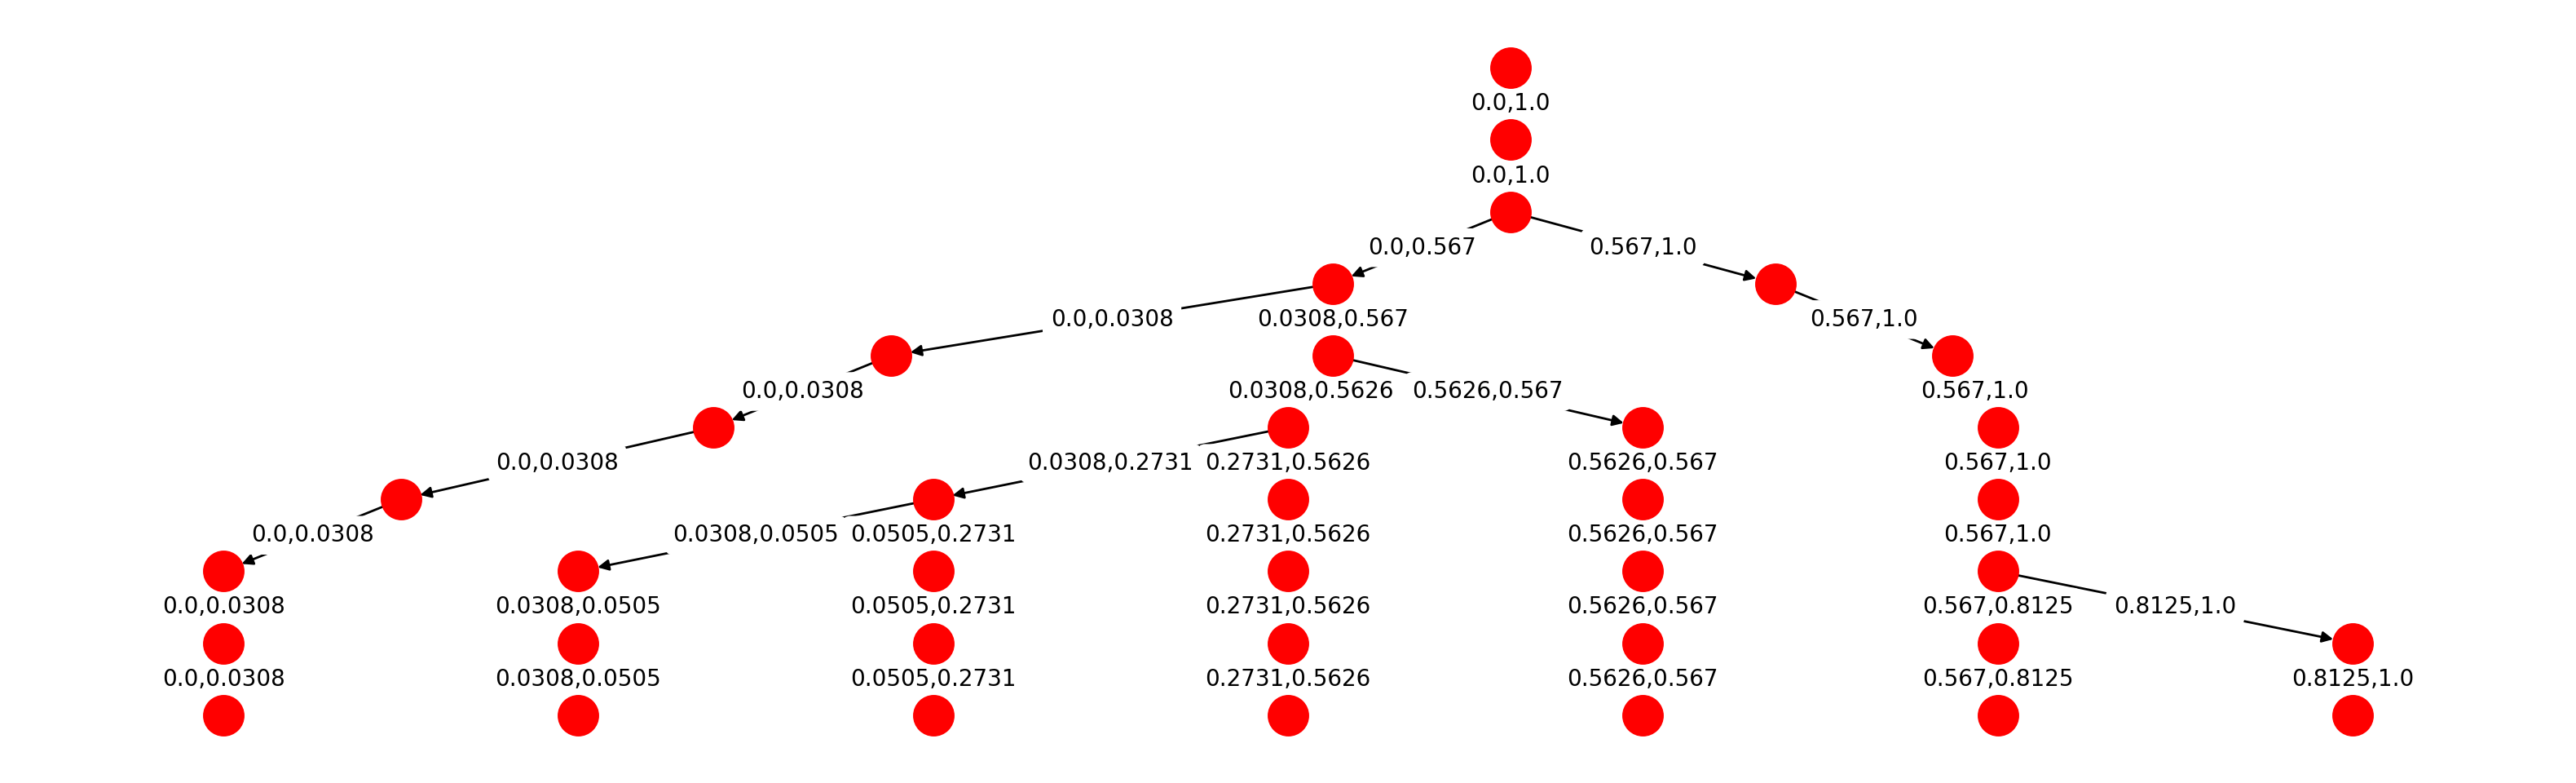
\includegraphics[width=\textwidth]{images/res_tree}
    \caption{Different values of $\alpha$ lead to different merges. We calculate a tree where we start with the entire range $[\alpha_{lo}, \alpha_{hi}]$ and split the interval into all different subintervals with consistent merges.}
    \label{fig:toe}
\end{figure}

We perform the described procedure for iterations $i = count(points) -1$ times until only one cluster containing all points is left. All the leaf nodes in the resulting tree of executions then represent one interval $[\alpha_{lo}, \alpha_{hi}]$ where the clustering is consistent within the interval and each interval contains a different clustering.\\

However just calculating the split values in a range $[\alpha_{lo}, \alpha_{hi}]$ does not necessarily yield to the best possible solution. One of these examples is demonstrated in figure \ref{fig:notoptimal}, where the blue line for the constant value of $d$ will not be considered, only the lines $\alpha \in [\alpha_{lo}, alpha_{split})$ (red) and $\alpha \in [\alpha_{split}, alpha_{high}]$ (black) will be.

\begin{figure}[H]
    \centering
    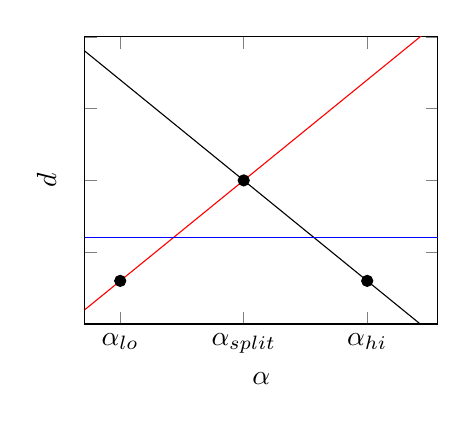
\begin{tikzpicture}
        \begin{axis}[ 
        xlabel=$\alpha$,
        ylabel={$d$},
        xmin=0.4,
        xmax=0.9,
        xtick={0.45,0.625,0.8},
        xticklabels={$\alpha_{lo}$, $\alpha_{split}$, $\alpha_{hi}$},
        width=0.5\textwidth,
        yticklabels={,,}
        ] 
        \addplot[mark=none, red] {-3+8*x}; 
        \addplot[mark=none, black] {-8*x+7};
        \addplot[mark=none, blue] {1.2};
        \addplot [only marks] table {
        0.45   0.6
        0.625  2
        0.8    0.6
        };
        \end{axis} 
    \end{tikzpicture}
    \caption{Simply calculating the split values between the start and the end value of the range $[\alpha_{lo}, \alpha_{hi}]$ will not necessarily lead to the optimal values. By doing so, the blue line (constant $d$ value) will not be considered.}
    \label{fig:notoptimal}
\end{figure}

In order to solve this, we can recursively check each resulting interval again if it contains different merging behaviors.

\begin{figure}[H]
    \centering
    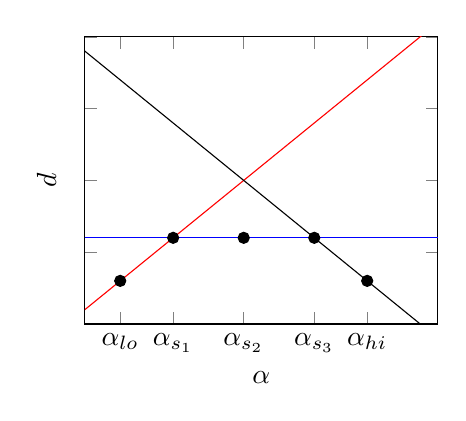
\begin{tikzpicture}
        \begin{axis}[ 
        xlabel=$\alpha$,
        ylabel={$d$},
        xmin=0.4,
        xmax=0.9,
        xtick={0.45,0.525,0.625,0.725,0.8},
        xticklabels={$\alpha_{lo}$, $\alpha_{s_1}$, $\alpha_{s_2}$, $\alpha_{s_3}$, $\alpha_{hi}$},
        width=0.5\textwidth,
        yticklabels={,,}
        ] 
        \addplot[mark=none, red] {-3+8*x}; 
        \addplot[mark=none, black] {-8*x+7};
        \addplot[mark=none, blue] {1.2};
        \addplot [only marks] table {
        0.45   0.6
        0.525  1.2
        0.625  1.2
        0.725  1.2
        0.8    0.6
        };
        \end{axis} 
    \end{tikzpicture}
    \caption{Simply calculating the split values between the start and the end value of the range $[\alpha_{lo}, \alpha_{hi}]$ will not necessarily lead to the optimal values. By doing so, the blue line (constant $d$ value) will not be considered.}
    \label{fig:notoptimal2}
\end{figure}

By calculating the split points recursively, the example in figure \ref{fig:notoptimal2} will result in the intervals $[\alpha_{lo}, \alpha_{s_1}]$, $[\alpha_{s_1}, \alpha_{s_2}]$, $[\alpha_{s_2}, \alpha_{s_3}]$ and $[\alpha_{s_3}, \alpha_{s_{hi}}]$. The optimal distance between $\alpha_{s_1}$ and $\alpha_{s_3}$ is covered now, but the results contain one unncessary interval as $\alpha_{s_2}$ still splits two intervals. The algorithm can check if older splits are still relevant, however the runtime cost to do so will be more expensive than carrying one additional interval with the same distance. We can use this knowledge and adapt algorithm \ref{alg:alphalinkage1}.

\begin{algorithm}[H]
    \KwData{input data $p_1, ..., p_N$, initial states $st$}
    \KwResult{$k$ intervals $[\alpha_0, \alpha_1], ..., [\alpha_{k-1},\alpha_k]$}
    \For{$iteration\gets1$ \KwTo $N-1$}{
        \ForEach{state $s \in st$}{%
        remove state $s$\;
        ranges $\gets$ find ranges between $s.\alpha_{lo}$ and $s.\alpha_{hi}$\;
        \ForEach{range $r \in ranges$}{%
                $cand \gets$ candidate for range\;
                $ms \gets$ merge $cand$\;
                add state $ms$ with range $r$ to the end of $st$\;
        }
      }
    }
    \caption{By calculating the split points between $\alpha_{lo}$ and $\alpha_{hi}$ recursively, we ensure that no optimal interval is left out.}
    \label{alg:alphalinkage2}
\end{algorithm}

As experimental results turn out to need a lot of memory (up to $\approx$ 20 GB for 300 points and 20,000 states), we want to adapt algorithm \ref{alg:alphalinkage2} so that it uses less memory. The memory usage scales relative to the amount of currently in-memory stored states, so the goal is to reduce these. As the amount of states is much larger than the amound of iterations, we calculate and evaluate the leave nodes of the tree and keep the alternative merges stored. This results in algorithm \ref{alg:alphalinkage3}.

\begin{algorithm}[H]
    \KwData{input data $p_1, ..., p_N$, initial states $st$}
    \KwResult{$k$ intervals $[\alpha_0, \alpha_1], ..., [\alpha_{k-1},\alpha_k]$}
    \While{$|st| > 0$}{
        \ForEach{state $s \in st$}{%
        remove state $s$\;
        \eIf{$s$ is final}{
          evaluate $s$\;
          }{
          ranges $\gets$ find ranges between $s.\alpha_{lo}$ and $s.\alpha_{hi}$\;
            \ForEach{range $r \in ranges$}{%
                    $cand \gets$ candidate for range\;
                    $ms \gets$ merge $cand$\;
                    add state $ms$ with range $r$ to the beginning of $st$\;
            }
         }
      }
    }
    \caption{Instead of calculating the nodes layerwise, this algorithm works pathwise, i.e. it goes down one path of a tree to a leaf node and evaluates it before continuing with the next split. This approach needs much less memory than the previous algorithms and has about the same runtime as shown in figure \ref{fig:performance}.}
    \label{alg:alphalinkage3}
\end{algorithm}

\begin{figure}[H]
\centering
\begin{minipage}{.45\textwidth}
  \centering
  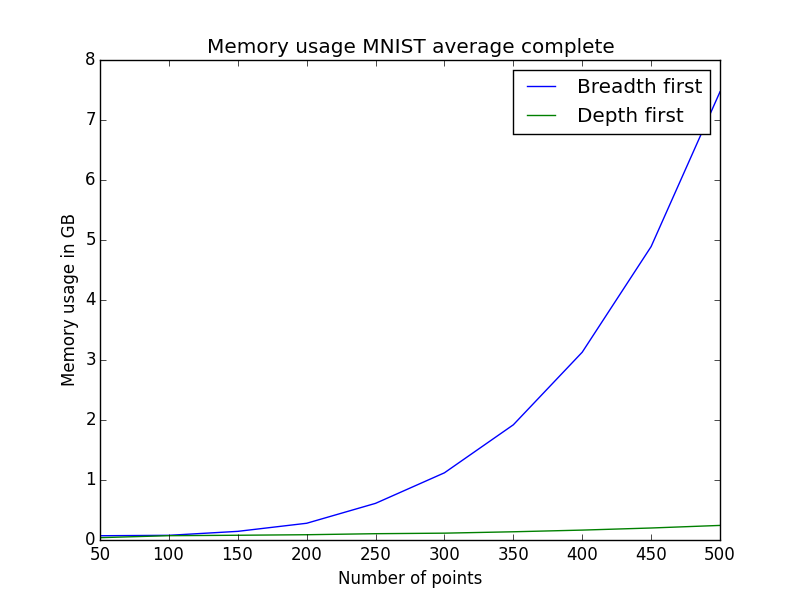
\includegraphics[width=\linewidth]{plots/memory_mnist_ac}
\end{minipage}\hfill
\begin{minipage}{.45\textwidth}
  \centering
  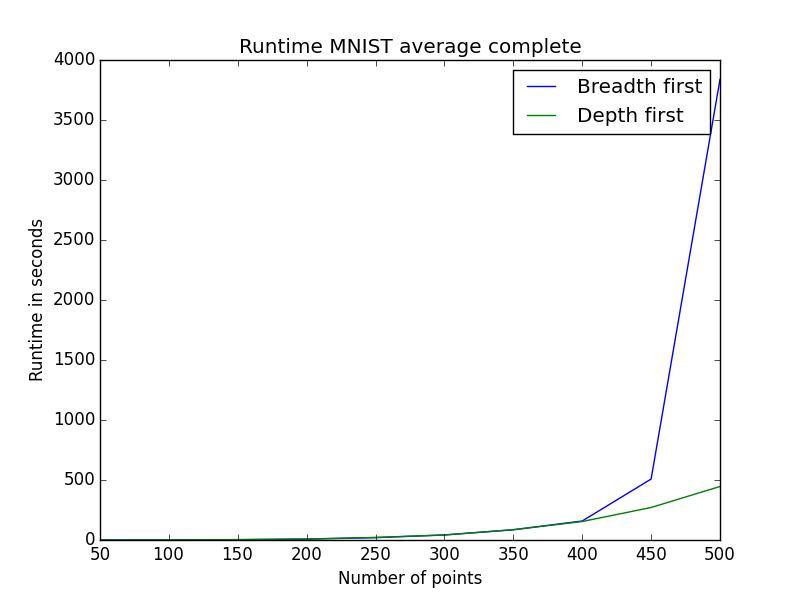
\includegraphics[width=\linewidth]{plots/runtime_mnist_ac}
\end{minipage}
\caption{The depth first implementation needs less memory and also has a better runtime compared to the breadth first implementation.}
\label{fig:performance}
\end{figure}

Instead of merging iteratively and steadily shrinking the intervals, we propose an algorithm with a geometric motivation. We are again evaluating an interval $[\alpha_{lo}, \alpha_{hi}]$, but we interprete the different merges as linear functions depending on $\alpha$. We can start by calculating the merge candidate for the start value $\alpha_{lo}$ and calculate the next intersection that will yield to the next merge. By calculating all the intersections of linear functions, we can also determine all the different intervals for the range $[\alpha_{lo}, \alpha_{hi}]$, where different merging behaviors occure. Algorithm \ref{alg:alphalinkage4} describes this procedure.

\begin{algorithm}[H]
    \KwData{input data $p_1, ..., p_N$, start value $\alpha_{lo}$, end value $\alpha_{hi}$}
    \KwResult{$k$ intervals $[\alpha_0, \alpha_1], ..., [\alpha_{k-1},\alpha_k]$}
    $\alpha \gets \alpha_{lo}$\;
    linear function $lf \gets$ get lf for alpha\;
    \While{$\alpha < \alpha_{hi}$}{
        $\alpha_{new} \gets$ calculate next split for $\alpha$\; 
        $lf \gets$ get lf for $\alpha_{new}$\;
        $\alpha \gets \alpha_{new}$
    }
    \caption{}
    \label{alg:alphalinkage4}
\end{algorithm}

\begin{figure}[H]
    \centering
    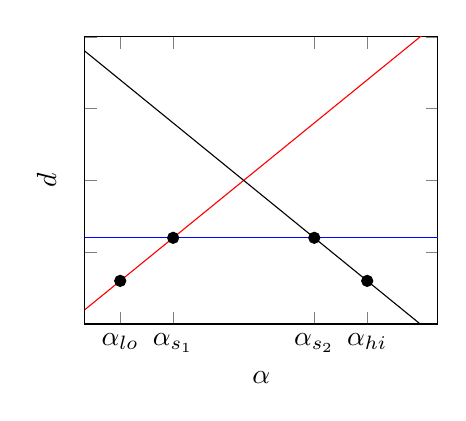
\begin{tikzpicture}
        \begin{axis}[ 
        xlabel=$\alpha$,
        ylabel={$d$},
        xmin=0.4,
        xmax=0.9,
        xtick={0.45,0.525,0.725,0.8},
        xticklabels={$\alpha_{lo}$, $\alpha_{s_1}$, $\alpha_{s_2}$, $\alpha_{hi}$},
        width=0.5\textwidth,
        yticklabels={,,}
        ] 
        \addplot[mark=none, red] {-3+8*x}; 
        \addplot[mark=none, black] {-8*x+7};
        \addplot[mark=none, blue] {1.2};
        \addplot [only marks] table {
        0.45   0.6
        0.525  1.2
        0.725  1.2
        0.8    0.6
        };
        \end{axis} 
    \end{tikzpicture}
    \caption{Simply calculating the split values between the start and the end value of the range $[\alpha_{lo}, \alpha_{hi}]$ will not necessarily lead to the optimal values. By doing so, the blue line (constant $d$ value) will not be considered.}
    \label{fig:optimal}
\end{figure}

\section{Performance Optimizations}

In order to have real-world applications, the proposed algorithms should run in an efficient way, i.e. it should not take the $\alpha$-linkage algorithms too much time to run. A first python implementation took days to run, but switching to C++ and using its advantages took down the runtime to hours. However, there are more optimization methods that we used in order to improve the runtime.

\subsection{Dynamic Programming}

One of the most time-consuming parts was the calculating of the distances. For each pair of clusters $C_i, C,j$ the distance had to be calculated for each clustering state. We optimized this by using dynamic programming and stored the distance matrices $D_{lower}$ and $D_{upper}$ for each state. The naming results from the different interpolation settings where we interpolate from one linkage distance (lower) to another linkage distance (upper), e.g. the setting in equation \ref{eq:singlecomplete} describes the interpolation from single linkage (lower) to complete linkage (upper). In this example we then store the pairwise distances for both single linkage and complete linkage and in order to find the merge candidates we have to do iterate over the distance matrices instead of calculating the distances over and over again. When we merge two clusters, we then update the distance matrices for the given state. Table \ref{dp:distances} shows an example for the pairwise distances of clusters $i$ and $j$.

\begin{table}[H]
    \centering
    \begin{tabular}{|l | l l l l l|}
    \hline
    j\textbackslash i & 0 & 1 & 2 & 3 & 4\\ \hline
    0 & 0 & 1.243 & 1.512 & 2.468 & 5.1243\\
    1 & 1.243 & 0 & 2.443 & 3.1412 & 4.443\\
    2 & 1.512 & 2.443 & 0 & 3.8988 & 6.827\\
    3 & 2.468 & 3.1412 & 3.8988 & 0 & 5.72\\
    4 & 5.1243 & 4.443 & 6.827 & 5.72 & 0\\ \hline
    \end{tabular}
    \caption{Storing the pairwise distances of all clusters avoids calculating the distances over and over again.}
    \label{dp:distances}
\end{table}

One observation that we can make is that the matrix has a lot of redundant values, because $D(i,j) = D(j,i)$. Removing these rendundant values will result in a trade-off between copying and indexing costs and will be discussed in the following section. Another optimization we can do is storing the indices of the active clusters, i.e. the clusters that can get merged. Once two clusters got merged, they cannot be merged any further, only the resulting cluster can. So we then do not have to consider the old clusters anymore and can remove them from the set of active indicies. This allows us to find the merge candidates faster as the pool of candidates gets smaller.

\subsection{Trade-Off between Copying and Indexing Costs}

Currently we can access the costs for a pair of clusters $C_i$ and $C_j$ through $D[i,j]$ or $D[i + j * width]$ for flattened matrices. These indices are very easy to calculate. In order to remove the redundant values from the distance matrix we remove all values below the diagonal as shown in table \ref{dp:distances2}.

\begin{table}[h]
    \centering
    \begin{tabular}{|l | l l l l l|}
    \hline
    j\textbackslash i & 0 & 1 & 2 & 3 & 4\\ \hline
    0 & 0 & 1.243 & 1.512 & 2.468 & 5.1243\\
    1 & \cellcolor{gray!25} & 0 & 2.443 & 3.1412 & 4.443\\
    2 & \cellcolor{gray!25} & \cellcolor{gray!25} & 0 & 3.8988 & 6.827\\
    3 & \cellcolor{gray!25} & \cellcolor{gray!25} & \cellcolor{gray!25} & 0 & 5.72\\
    4 & \cellcolor{gray!25} & \cellcolor{gray!25} & \cellcolor{gray!25} & \cellcolor{gray!25} & 0\\ \hline
    \end{tabular}
    \caption{Storing the pairwise distances of all clusters avoids calculating the distances over and over again.}
    \label{dp:distances2}
\end{table}

In addition to that we can also remove the diagonal values as they represent the distances between the same clusters and are thus always zero. This results in table \ref{dp:distances3}.

\begin{table}[H]
    \centering
    \begin{tabular}{|l | l l l l l|}
    \hline
    j\textbackslash i & 0 & 1 & 2 & 3 & 4\\ \hline
    0 & \cellcolor{gray!25} & 1.243 & 1.512 & 2.468 & 5.1243\\
    1 & \cellcolor{gray!25} & \cellcolor{gray!25} & 2.443 & 3.1412 & 4.443\\
    2 & \cellcolor{gray!25} & \cellcolor{gray!25} & \cellcolor{gray!25} & 3.8988 & 6.827\\
    3 & \cellcolor{gray!25} & \cellcolor{gray!25} & \cellcolor{gray!25} & \cellcolor{gray!25} & 5.72\\
    4 & \cellcolor{gray!25} & \cellcolor{gray!25} & \cellcolor{gray!25} & \cellcolor{gray!25} & \cellcolor{gray!25} \\ \hline
    \end{tabular}
    \caption{Storing the pairwise distances of all clusters avoids calculating the distances over and over again.}
    \label{dp:distances3}
\end{table}

The matrices are now smaller, so they need less memory. In the example, we changed a matrix of the size $25$ to a matrix of the size $10$. In general a matrix of the size $n$x$n$ will be compressed to a matrix of the size $\frac{n^2-n}{2}$. The lower amount of needed memory also results in less copying costs that will lead to a better runtime. However, the indexing is not as easy anymore. For easier storage, we again work with flattened matrices, the indexing for the resulting list is shown in equation \ref{eq:indexing}.

\begin{equation}
    \begin{aligned}
        index(i,j) = \frac{width * (width - 1)}{2} - \frac{(width - j) * (width - j - 1)}{2} + i - j - 1
    \end{aligned}
    \label{eq:indexing}
\end{equation}

Calculating this index in a nested loop is very expensive, however we calculate the part that does not depend on $i$ in the outer loop and thus only need to add $i$ in the inner loop. This does not only yield to a lower memory usage of $\approx 30\%$, but also increases the runtime by TODO.

\todo[inline]{runtime improvement factor}

\subsection{Implementation-specific Optimizations}

In order to optimize the implementation even further, we will have a look into the implementation. One optimization that already was briefly described is the flatterning of the matrices, so the resulting list will be one-dimensional and can be iterated easier and faster.\\

Another observation is that copy operations are computationally expensive, so we avoid them as much as possible. In the described algorithms (\ref{alg:alphalinkage1}, \ref{alg:alphalinkage2} and \ref{alg:alphalinkage3}) we removed a state from the list of states and added other states. In an optimized way, we do not remove the state and just overwrite the state with the resulting state. Once there are splits in the current interval, the state gets overwritten and additional states get added to the list.\\

We can also optimize the way of updating the distance matrices. Instead of adding new clusters there for a merge of clusters $i$ and $j$ we update the distances of $i$ to all active clusters with the distances of the resulting cluster. The distances of the cluster $j$ will not be considered for merges anymore as the index $j$ gets removed from the active indices. This has the advantage that the size of the distance matrices will not increase after merges.\\

Also, the data types make an important contribution to the memory usage. Instead of using double precision floating point values, single precision is enough to clearly identify and separate all the resulting intervals. Same goes for the distances as we only need the minimum and maximum distances, that are not effected by loss of precision. To store the indices of the clusters, we know that they will not exceed $2^{16}$, so they can be store as half precision values.